\documentclass[10pt]{report}
\usepackage[margin=.5in]{geometry}
\usepackage{graphicx}
\usepackage{array,booktabs,ragged2e,ctable,enumitem}
\usepackage{multirow,textcomp}
\usepackage{lastpage}
\usepackage{fancyhdr}

\fancyfoot[C]{Page \thepage\ of \pageref{LastPage}}


\newcolumntype{L}[1]{>{\raggedright\let\newline\\\arraybackslash\hspace{0pt}}m{#1}}
\newcolumntype{C}[1]{>{\centering\let\newline\\\arraybackslash\hspace{0pt}}m{#1}}
\newcolumntype{R}[1]{>{\raggedleft\let\newline\\\arraybackslash\hspace{0pt}}m{#1}}
%opening
%\title{}
%\author{}


\renewcommand{\headrulewidth}{0pt} 
\pagestyle{fancy}


\begin{document}


{
\setlength{\arrayrulewidth}{.4em}

\noindent
\begin{table}
\begin{tabular}{ L{5em} L{.5\textwidth}  R{.35\textwidth} }
\hline
\multirow{2}{*}{
	%\begin{figure}
	%\centering
	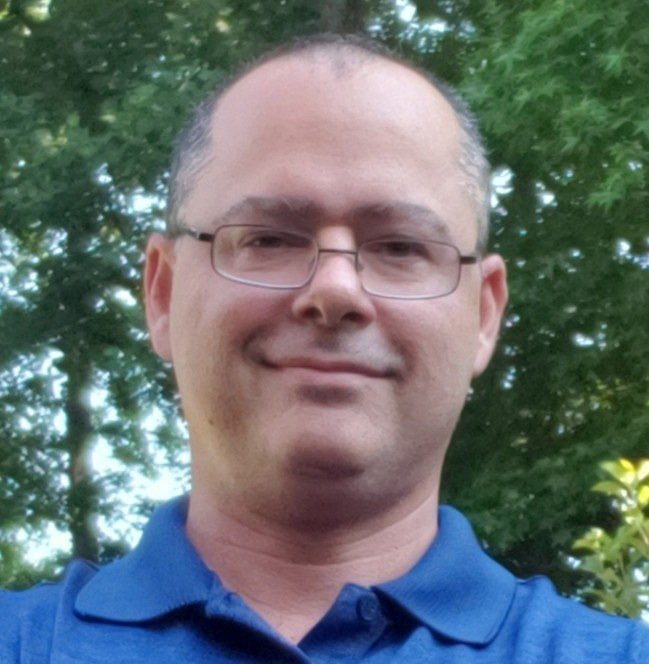
\includegraphics[width=0.75\linewidth]{./sdm-2021-photo.jpeg}
	%\end{figure}
}
& \textbf{Stephen D. Mathews} & \textbf{Director IT/Sr. Application Analyst} \\
& 4320 Chatham View Dr. Buford, GA 30518 & Mobile: (954) 649-9681 \\
& \textsl{busysteve@gmail.com} &   \\
\hline
\end{tabular}
	\center
	\textsl{``Always looking forward to what I enjoy doing most...} \\
	\textsl{...Solving problems.''}
	\begin{quote}
		\begin{quote}
			Stephen enjoys solving big problems with simple solutions. His experience speaks for itself as he has taken part in providing many solutions for various needs. His passion for his work is as obvious as the joy he receives from it. He cares about others as he strives to exceed the expectation of his superiors and coworkers.
		\end{quote}
	\end{quote}
\end{table}
}


%\maketitle
%\begin{abstract}
%\end{abstract}

\setitemize{itemsep=0pt}

\vspace{-5em}

\section*{Qualifications:}

\begin{itemize}

\item Thirty+ years of programming experience (including childhood starting in 1984)
\item Twenty five years of professional programming experience in C and C++
\item Regularly use modern C++ concurrency features and employ many features offered in C++17 
\item Twenty years financial payments processing experience
\item Front End Authorization and Back End Settlement for Debit and Prepaid processing
\item UNIX and Windows software development using C++
\item High Performance On Line Transaction Processing systems design and development
\item Multi-platform system development
\item Embedded development using Linux and proprietary operating systems and platforms
\item Cryptographic network application security using well known algorithms, protocols, and APIs
\item Use of cross platform (Windows/UNIX) open source C++ GUI libraries such as Qt and FLTK
\item Database layout and application design and development with many databases (such as DB2, SQL Server, Oracle, MySQL, SQLite, MongoDB) using SQL, native database APIs such as OCI and CLI
\item Real-time development of embedded micro-controllers
\item Business process analysis for streamlining, automation, and data handling/processing
\item Business accounting analysis and development experience
\item Follow Common Software Development Life Cycles (SDLC)
\end{itemize}


\subsection*{Leadership}
\begin{itemize}
	\item Streamline many development processes/projects through resource management
	\item Able to efficiently manage and apply the skills of both experienced and inexperienced developers on the same team to meet objectives
	\item Able to manage effectively regardless of personality types
	\item Commonly dealt with both mixed language and mixed platform development environments
	\item Always able to take suggestions from anyone
	\item Believe that high morale leads to high creativity and productivity
\end{itemize}


\section*{Operating Systems:}

\begin{math}
\large
\textrm{ Linux }
\bullet \space \textrm{ AIX } \space
\bullet \space \textrm{ Windows } \space
\bullet \space \textrm{ Solaris } \space
\bullet \space \textrm{ MacOSX } \space
\bullet \space \textrm{ HP/UX }
\end{math}

\pagebreak

\section*{Programming Experience:}

\subsection*{C/C++(17):}


\begin{itemize}
\item Cross platform project development of Client and Server software for UNIX/Linux and Windows supporting multiple compilers (e.g. GCC, XLC, and Visual C++)
\item Make use of polymorphism in designs when applicable to provide scalability and abstractions from various subsystem details (e.g. Multiple native database APIs, Mixed intercommunication link adapters, B2B integration, System I/O)
\item Designing template classes and use many classes of the STL
\item Utilized Boost before C++11 for many of the feature brought into C++
\item Designed and developed easy-to-use class libraries with exception handling used as wrappers of system level functions (e.g. Socket communication and Device Access), encryption algorithms (e.g. RSA, AES, RC4, DES, MD5, etc...) and API’s (i.e. OpenSSL), 2D graphics handling, and business logic 
%\item Writing classes and COM wrappers of various APIs for C++, VC++ and Visual Basic development
\item Designing and developed high availability secured transaction oriented systems on multiple platforms natively
\item Designed and developed real-time enterprise system monitoring infrastructure
\item B2B; Bridging legacy systems to modern systems with common and custom protocols
\item Embedded system design and development for a variety of applications
\item Developed high speed parser classes for high volumes of XML, delimited, and fixed width data
\end{itemize}


\subsection*{R \& RStudio}
\begin{itemize}
\item Statistically based system alerting to predict the on set of problems 
\item Trend analysis and capacity planning
\item General statistical study of business telemetry
\item Analysis of Data in stores of DB2, Oracle, MongoDB, Spark and file systems
\item Analysis of Splunk data via REST calls
\end{itemize}

\subsection*{DB2 / Oracle / MongoDB / SQL Server / Sybase / MySQL / SQLite}
\begin{itemize}
	\item Server design and database layouts, setup security and automated maintenance
	\item Work with ODBC and native API
	\item Extensive knowledge of SQL both standard and native
	\item Use of native APIs such as DB2 CLI, NTWDBLIB/FreeTDS, OCI, mysql.lib
\end{itemize}

\subsection*{Awk}
\begin{itemize}
	\item Use for general utility scripting 
	\item Automated system statistics reporting
	\item Preprocessing of file from specialize applications
	\item Parsing and transforming of data
\end{itemize}


\subsection*{Java}
\begin{itemize}
%\item Developed browser based client applications using applets
\item Developed back-end services for corporate system monitoring
\item Used for multi-platform GUI applications and for transaction based server development
\item Integrated Java with other systems in a distributed environment using TCP/IP
\end{itemize}

%\subsection*{Web / HTML / JavaScript}
%\begin{itemize}
%\item Designed web sites with pages offering content validation, frames, tables, etc.
%\item Developed graphics and animations
%\item Interactive interfaces with JavaScript
%\item Created web based interfaces to legacy systems for inventory queries, order placement, and data access
%\end{itemize}


\pagebreak

\section*{Work Experience ---}

\noindent
\begin{tabular}{ L{.5\textwidth}  R{.4\textwidth} }
\textbf{\large First Data Corp. now Fiserv} & 9/2009 -- Present \\
Director IT \& Sr. Application Analyst &
\end{tabular}


\begin{itemize}
\item Designed and Developed a mission critical system-wide processing engine in C++ for First Data's Smart Routing
\item Develop transaction analysis models for internal and client use
\item Designed and developed and latency aware service pooling template class set for Databases, REST APIs, SOA Services, and transaction systems
\item Well versed in Splunk and a certified Power User
\item Built and maintain distributed monitoring facility before we bought Splunk that is still in use
\item Subject Matter Expert for Debit processing and Debit Network Least Cost Routing
\item Application Architect for debit processing systems
\item Author of process to handle implications of the Durbin amendment to the Dodd-Frank Wall\textsuperscript{\tiny St} Reform
\item Author of First Data's TransArmor\textsuperscript{\tiny TM} Monitoring Backend
\item Commonly write utilities for time saving, load testing, and data management
\end{itemize}
\bigskip

\noindent
\begin{tabular}{ L{.5\textwidth}  R{.4\textwidth} }
\textbf{\large FIS / eFunds / Wildcard System, Inc.} & 3/2002 -- 9/2009 \\
Sr. Application Analyst &
\end{tabular}

\begin{itemize}
\item Part of the Data Center Systems team as senior business systems analyst/developer and a financial settlement processing subject matter expert.  
\item Design and develop multiplatform enterprise level real-time monitoring system in C++ for support and management staff use. 
\item Lead a team of developers in backend systems development and maintenance
\item Have also been tasked with personally leading the design and development of a business intelligence system that is now live but still evolving.
\item Maintain, enhance, troubleshoot, repair and optimize processes and data used for settlement processing.
\item Mining of data for research, auditing and troubleshooting.
\item Expanded internal charge back system ASP interface to support Visa international charge back exhibit forms.
\item Rewrote MasterCard settlement batch loaders with one other team member to support GCMS (ISO-8583) update in Java reusing existing code to meet short deadline.
\item One of the few authors of SQL Server Extended Stored Procedures in the company using C/C++.
\end{itemize}
\bigskip

\noindent
\begin{tabular}{ L{.5\textwidth}  R{.4\textwidth} }
\textbf{\large Tangent Associates, Inc.} & 11/2001 -- 3/2002 \\
POS Application Developer
\end{tabular}

\begin{itemize}
\item Was hired primarily to design, develop and implement the Stadium POS system industry’s first fully TCP/IP based POS system in C++ for embedded systems in a very short time.
\item Developed centralized POS station management service software for Windows and Linux servers.
\item Led development of embedded POS station software for StrongARM Linux using GCC.
\item Designed a custom fully automatic configuration protocol based on the DHCP and BOOTP specifications to reduce the needed knowledge base of the client’s network administrators.
\item Designed redundant self updating subsystem for the POS station software for central deployment of software updates
\end{itemize}
\bigskip

\noindent
\begin{tabular}{ L{.5\textwidth}  R{.4\textwidth} }
\textbf{\large Wildcard System, Inc.} & 8/2001 -- 10/2001 \\
Application Analyst
\end{tabular}

\begin{itemize}
\item Assisted in complete redesign of reporting system front and backend used by the company; The system was designed to use any database and run on Windows with later intent for UNIX migration.
\item Wrote a parser in C++ to read a large number of existing Perl reports and reporting utility scripts; The parser was used to migrate all embedded queries and hard coded data used for reporting to the newer dynamic architecture.
\end{itemize}
\bigskip

\noindent
\begin{tabular}{ L{.5\textwidth}  R{.4\textwidth} }
\textbf{\large Innerhost, Inc.} & 2/2001 -- 8/2001 \\
Software Developer
\end{tabular}

\begin{itemize}
\item Assisted in analysis of business software requirements for billing, A/R, and collections.
\item Implemented custom business policies to Portal Software\textquotesingle s Infranet billing system used at iNNERHOST
%\item Designed and developed desktop and server applications used internally to simplify the setup of shared web hosting accounts for customers using Visual Basic and C++ COM components
%\item Designed and developed COM client components that were plugged into ASP pages allowing customers to setup a web hosting accounts that were allocated and activated on the web servers on in real-time.
\end{itemize}
\bigskip


\noindent
\begin{tabular}{ L{.5\textwidth}  R{.4\textwidth} }
\textbf{\large Dynamic Imaging, Corp.}  & 8/1998 -- 2/2001 \\
Head of Research and Development &
\end{tabular}

\begin{itemize}
\item Established complete plan and process for multi-platform development of entire product suite.
\item Designed standard processes for documenting, designing, and developing all software products.
\item Wrote a multi-platform polymorphic database API wrapper that encompassed all major native database APIs for an average performance benefit over ODBC of about twenty percent.
\item Developed training for new hires in multi-platform development methods.
\item Personally responsible for all cryptographic security measures developed and implement in the enterprise class suite this included SSL communication, custom protocols based well known algorithms, certificate generation, and security auditing of client’s internal and external network infrastructure.
\item Consulted with clients on how they could implement or improve the security of their infrastructure from internal and external invasions with the lowest cost and simplest practices, for both Windows and UNIX systems.
\item Designed and developed a multithreaded digital image storage/retrieval server that compiled on UNIX and Windows from the same C++ source code.
\item Established Qt (www.trolltech.com) as the GUI tool kit of choice for our product suite.
\item Developed performance monitoring tools using FLTK (www.fltk.org) due to improved graphics support.
\item Wrote many custom applications for customers using MFC, Visual Basic, or Qt depending on their needs.
\item A complete set of toolkits/APIs was developed to allow customers and VARs to customize the look and feel of our document imaging product suite, these tools were in the form of COM/ActiveX components, CORBA components, C libraries, and C++ classes.
\item The web product was designed to run as a stand alone server it was written primarily in C++ for high speed image rendering and conversion and used JSP to handle basic session management.
\item The entire document imaging product suite ran natively on many platforms and used encrypted XML bundles on top of TCP/IP as its primary method of communication between all of our products.
\item Also wrote a single pass XML parser that allowed for midstream parsing of XML data mixed with RAW binary data.
\end{itemize}
\bigskip


\noindent
\begin{tabular}{ L{.5\textwidth}  R{.4\textwidth} }
\textbf{\large The Maxim Group}  & 5/1998 -- 8/1998 \\
Software Developer(Short-term Contractor) &
\end{tabular}

\begin{itemize}
\item Conducted analysis for porting an international development effort (30+ developers and three backend Web products) from Win32/MFC to a UNIX environment in C++ using NSAPI or raw CGI.
\item Designed and implemented multi-platform internet protocol wrapper classes in C++.
\item Demonstrated suggested approaches for multi-platform development based on analysis.
\item Worked with the team on general web development tasks for their travel reservation system.
\end{itemize}
\bigskip

%\pagebreak

\noindent
\begin{tabular}{ L{.5\textwidth}  R{.4\textwidth} }
\textbf{\large Advanced Information Technologies}  & 10/97 -- 5/98 \\
Software Developer &
\end{tabular}

\begin{itemize}
\item Worked on Design and development of a corporate service/repair and dispatch system for BrandsMart USA Service Center in a team environment complete with logistics support for parts inventory/usage tracking with the combined use of Visual Basic and C++.
\item Multilanguage environment allowed for development of COM components using ATL to handle common transactions for speed and Visual Basic to host the components and for the GUI development based on the required business logic of the company.  This was before VB supported component development.
\item Developed custom applications on an as needed basis in Visual Basic and Visual C++.
\item Assisted in Writing of design, technical, and user documentation.
%\item Assisted in port of a legacy application used in Collier County Property Appraiser’s office to VB.
\end{itemize}
\bigskip



\noindent
\begin{tabular}{ L{.5\textwidth}  R{.4\textwidth} }
\textbf{\large State of FL, Dept. of Community Affairs}  & 9/96 -- 10/97 \\
Systems Analyst/Developer &
\end{tabular}

\begin{itemize}
\item Coordinated migration from Novell based systems to Windows NT.
\item Developed custom software in Visual C++ for the transfer of large amounts of data for the migration effort.
\item Acted as a liaison for migration issues between the State and FEMA (Federal Emergency Management Agency).
\item Wrote user and technical documentation
\item Trained employees on the use of custom applications to repair corrupted data in the Novell System.
\item Provided support to employees for custom and legacy applications.
\item Defined the structure and security used for the new Windows NT network.
\end{itemize}
\bigskip

\noindent
\begin{tabular}{ L{.5\textwidth}  R{.4\textwidth} }
\textbf{\large R/M Equipment, Inc.}  & 8/94 -- 9/96 \\
CNC Programmer / Assistant Prototyping Machinist / Weapons Specialist &
\end{tabular}

\begin{itemize}
\item Designed mass production manufacturing processes for military and local authority weapons accessories.
\item Developed software for computer automated mass production machinery.
\item Designed and machined custom holding fixtures to increase production efficiency of M203PI grenade launchers.
\item Developed embedded software for 8-bit micro controllers in C and assembler for prototype systems.
\item Interfacing software for the micro controllers was developed in Visual C++ 1.5.
\item Redesigned and machined many first run prototypes for field testing.
\item Made daily use of mathematics in mechanical and software design for trajectory calculations and curves.
\item Responsible for all technical, design, and research documentation  
\end{itemize}
\bigskip

\noindent
\begin{tabular}{ L{.5\textwidth}  R{.4\textwidth} }
\textbf{\large Harris Lanier}  & 1989 -- 1994 \\
Technician / Programmer &
\end{tabular}

\begin{itemize}
\item Custom software development for clients in C
\item Presentation and documentation management software development
\item Component level repair of electronic office equipment such as presentation systems, micro fiche readers and copiers
\item Submitted electronic update proposals for review and implementation into production equipment
\end{itemize}
\bigskip
\bigskip


\noindent
\begin{tabular}{ L{.5\textwidth}  R{.4\textwidth} }
	\textbf{\large Personal Research Studies}  &  \\
	 &
\end{tabular}

\begin{itemize}
	\item Modern C++ -- Working towards becoming a better user of C++
	\item GPU -- Learning how to incorporate the power of GPUs in practical ways	
	\item Machine Learning -- As applied to Data Analytics
	\item Analysis -- Learning and refining analytical skills
	\item Applied Statistics -- As applied to trend analysis and performance tuning
	\item Generics -- Increasing my understanding of applied generic programming
\end{itemize}
\bigskip


\noindent
\begin{tabular}{ L{.5\textwidth}  R{.4\textwidth} }
	\textbf{\large Personal Interests}  &  \\
	&
\end{tabular}

\begin{itemize}
	\item Computing -- I always enjoy learning more about computing than I already know	
	\item Biblical Greek -- Because it is challenging and insightful
	\item Boating -- Nice to unwind on the lake
	\item Metal \& Wood Crafting -- I was once a machinist and enjoy it
	\item Mt. Biking -- Raced, but not anymore, now just for fun
	\item Amateur Radio -- Extra Licensed : Call sign K4SDM
	\item Arduino -- I love finding ways to have an Arduino make life easier
\end{itemize}
\bigskip



%\section*{References}
%\center{
%References available upon request
%}



\vfill

\center



{Authored by hand in \LaTeX\ by Stephen Mathews}


\end{document}
